In this section, we will apply the structural results of the barrier forming problem and provide effective method to tackle it.
First, we start with a general method for obtaining the optimal solution among a set of candidate barriers.
Then, based on different ways to generate the candidate barriers, two approaches are given while one is based on 
using bitangent line segments and the other is based on sampling.

\subsection{Optimal Solution for Given Line Separator Candidates}
\label{sec:algo:ilp}
In the barrier forming problem, if the candidate barriers are available as a finite set, we can tackle the problem with integer programming (IP). 
To solve it, we first perform a decomposition of the workspace using the candidate barriers, which partitions the workspace into cells whose edges are part of some candidate barriers. 
Denote  $N$ as the number of candidate barrier line segments, and $M$ as the number of 
cells dissected using the candidate barriers. Fig.~\ref{fig:ilp_example} shows an example of dissecting the workspace into six cells with three candidate barriers.
Then, we can start to construct an IP model to solve the problem of minimizing the number of selected barriers. 
First, we use $\lceil\log k\rceil$ binary variables for each cell, 
resulting in $M\cdot\lceil \log k \rceil$ such variables $c_{11}, \dots, c_{M\lceil\log k\rceil}$. 
The value of $\overline{c_{i1}c_{i2}\dots c_{i\lceil \log k\rceil}}$ will represent the class of cell $i$. 
Thus, if there is an object in cell $i$, $\overline{c_{i1}c_{i2}\dots c_{i\lceil \log k\rceil}}$ should have a fixed value according to the class of the object.
A binary variable for each candidate line segment is used to indicate whether that line candidate is selected,
resulting in $N$ such variables: $\ell_1, \dots, \ell_N$. 

\begin{figure}
    \centering
    \begin{overpic}[width=0.3\textwidth]{chapters/bc/fig/ilp_example.png}
    \put(0, 60) {$\ell_1$}
    \put(40, 95) {$\ell_2$}
    \put(55, 95) {$\ell_3$}
    
    \put(15, 80) {$c_1$}
    \put(50, 75) {$c_2$}
    \put(80, 80) {$c_3$}
    \put(15, 30) {$c_4$}
    \put(50, 15) {$c_5$}
    \put(80, 30) {$c_6$}
    \end{overpic}
    % \includegraphics
    \caption{In this example, we aim to separate two groups of objects with the given candidate barriers. The workspace is decomposed into 6 cells by the 3 candidate barriers. As an example of constraint setup, the pair of adjacent cells $c_1$ and $c_4$ create a constraint of
    $\ell_1\geq c_1 \oplus c_4$, which is equivalent to $\ell_1\geq c_1 - c_4 \wedge \ell_1\geq c_4 -c_1$. (Since there is only $k=2$ classes of objects and $\log k =1$ here, the second index of $c_{i*}$ is eliminated.)} 
    \label{fig:ilp_example}
    \vspace{-0.2in}
\end{figure}

Between each pair of adjacent cells $i$ and $ j$ (let the candidate line segment between them correspond to $\ell_\sigma$), we have ($\oplus$ denotes ``exclusive or'')
\begin{equation}
\begin{split}
    &\ell_\sigma \geq c_{i\tau} \oplus c_{j\tau}  \Leftrightarrow \ell_\sigma \geq c_{i\tau} - c_{j\tau} \wedge \ell_\sigma\geq c_{j\tau} - c_{i\tau}, \\
    &\text{  for each adjacent cell $i$, $j$, and $1\leq \tau \leq \lceil \log k \rceil$},
\end{split}
\end{equation}
which means if two adjacent cells belong to different classes, then the line segment candidate between them must be selected. An example of the constraint setup is illustrated in Fig.~\ref{fig:ilp_example}.
Naturally, we have fixed $c_{i1},\dots,c_{i\lceil \log k\rceil}$ if ceil $i$ contains an object to be separated, and the value of $\overline{c_{i1}c_{i2}\dots c_{i\lceil \log k\rceil}}$ is set to be the same as its class index: $0\sim k-1$.
The objective is set to minimize the total number of line candidates selected, i.e., $\min \sum_{i=1}^{M} l_i$.

\subsection{Near-optimal Solution Using Bitangent Lines}
As the results in Section~\ref{sec:structure} show, using bitangent line segments 
can always provide optimal solution for the problem of barrier forming for point objects, 
and at least 2-OPT
solution for separating polygonal objects. 
Since the number of bitangent line segments is at 
most quadratic to the number of object or obstacle vertices, 
we can enumerate them, and apply IP method in Section~\ref{sec:algo:ilp} to find a solution. Fig.~\ref{fig:barrier_candidates} illustrates the candidate barriers constructed for point objects and polygonal objects.
It is worth noting that for enumerating bitangent barriers for point objects, the side of the point to the barrier also matters. For example, a pair of point objects will create $4$ bitangent barrier candidates as there are 4 different possible cases depending on the how the corresponding objects are placed with respect to the line. 

\begin{figure}[ht]
    \centering
    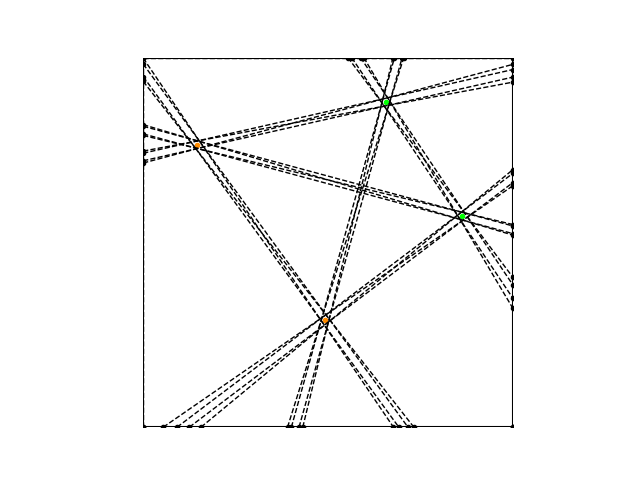
\includegraphics[trim=80 20 80 20,clip, width = .24\textwidth]{chapters/bc/fig/candidate_1.png}
    \hspace{-.1in}
    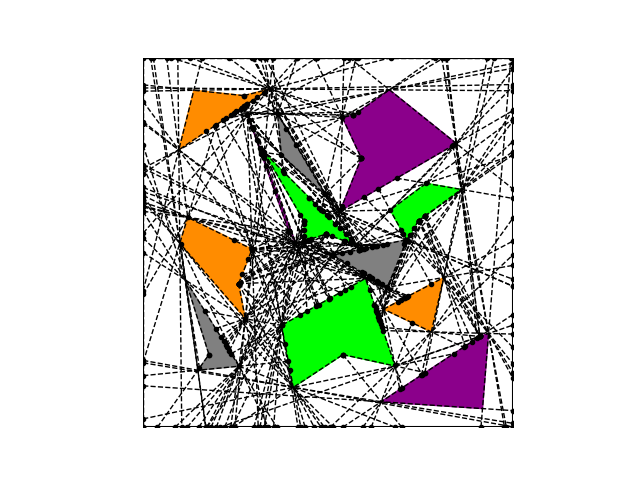
\includegraphics[trim=80 20 80 20,clip, width = .24\textwidth]{chapters/bc/fig/candidate_2.png}
    \caption{Illustration of bitangent barrier candidates. The left picture shows the bitangent
    candidates for $2$ point sets, each with $2$ points. In this case, a pair of points will create $4$ candidates. We note that we made the points non-zero-dimensional for visibility purposes. The right picture shows the bitangent candidates for $12$ polygonal objects in four sets.}
    \label{fig:barrier_candidates}
\end{figure}

\subsection{Sampling-based Resolution Complete Algorithm}
Although using bitangent line segments works well in most of the cases, it unfortunately cannot provide an optimal guarantee for the barriers formed when dealing with polygonal objects.
However, theorem~\ref{theorem:sin_tan} provides a good starting point for sampling line segments: we may limit candidate barrier sets to single tangents, i.e., we sample line segments passing through each object vertex in a radial manner. Hence, if we gradually increase the sampling resolution around each object and obstacle vertex and use the sampled line segments as candidate barriers, we can guarantee the asymptotic optimality of the resulting solution.

% In this section, we first describe a polynomial time approximation algorithm for a restricted version of Problem~\ref{p:2}. Then, we describe a general integer linear programming framework for solving Problems~\ref{p:1}-\ref{p:3},
% and local improvement techniques for enhancing solution quality.

% \subsection{Polynomial Time Approximation Algorithm}
% % Briefly mention the hardness results
% % As for 2D OSG, it is similar to the metric k-center problem and therefore
% the approximation algorithms solving k-center problem can be applied to 2D OSG. 

In their general forms, Problems~\ref{p:1}-\ref{p:3} require the computation of 3D visibility, a hard task on its own. Due to this reason, a polynomial time algorithm with guaranteed good approximation ratio for these problems appear difficult to come by. It is an interesting question to ask whether some form of approximation scheme can be derived. Here, we show that for Problem~\ref{p:2}, if one relax the visibility requirement, i.e. letting $vis(\cdot, \cdot)\equiv 1$, then a polynomial time $(2+\varepsilon)$-approximation algorithm can be obtained. 

Taking Problem~\ref{p:2}, we examine a setup assuming that each point $p \in S$ has good visibility, i.e., $p$ is always visible to the nearest sensor. Such scenarios happen when the 3D domain does not have large curvatures that would easily block sensors' view, e.g., covering the earth with GPS satellites or using drones to survey a vineyard. To drive a specific approximation bound, 
we further assume that sensors have spherical range sensing and are in a plane of some fixed 
\begin{wrapfigure}[5]{r}{1.3in}
  \vspace*{0mm}
  \begin{overpic}[width=1.3in,tics=5]{chapters/surf/fig/env.png}
	\end{overpic}
\vspace*{-6.5mm}
\end{wrapfigure}
height $h$ from the ground, which may be relaxed. Denote this surface as $H_C$. 
The figure on the right provides an illustration of the target environment setting. 

The main idea is to first obtain a dense sample of $S$ and then adapt $2$-approximation algorithms for the corresponding 2D setting, which requires some non-trivial reasoning. Two well-known approximation algorithms for $k$-center like problem in 2D are based on \emph{farthest point clustering} \cite{gonzalez1985clustering} and \emph{dominating set} \cite{hochbaum1985best, vazirani2013approximation}. Both of these approaches work for our purpose; we show how to work with the former.

Let a uniformly sampled set of point of $S$ be $S_N = \{o_1, \ldots, o_N\}$. We apply farthest point clustering \cite{gonzalez1985clustering} on $S_N$ as follows. As the name suggest, it picks farthest sensor locations until the number of sensors are exhausted. In the original approach, the points to be clustered are also sensor locations, which is not true here. Instead, we perform clustering in the set $S_N$ and project the selected samples to $H_C$ gradually. The relatively straightforward process is given in Algorithm~\ref{alg:greedy} (($d(\cdot$,$\ \cdot)$ denotes the distance between the inputs, one or both of which may be sets).


\begin{algorithm}
\begin{small}
    \SetKwInOut{Input}{Input}
    \SetKwInOut{Output}{Output}
    \SetKwComment{Comment}{\% }{}
    \caption{Farthest Point Clustering}
		\label{alg:greedy}
    \SetAlgoLined
		\vspace{1mm}
    \Input{$S_N$=\{$o_1, \dots, o_N$\}: $N$ sampled points on the surface $S\subset \partial \mathcal E$; $k$: number of sensors;\\
    $H_C$: a plane with a fixed height}
    \Output{$\mathcal{C}$: sensor location set}
		\vspace{1mm}
        % $\mathcal C$ = $\varnothing$\\
        $\mathcal{C} \leftarrow$  \{$o_1$'s vertical projection onto $H_C$\}\\
        % \While{$|\mathcal{C}|<k$}{
        \For{$i \gets 1$ \KwTo $k$}{
        \For{$o\in S_N$}{
        compute the distance $d(o, \mathcal{C})$ between $o$ and $\mathcal{C}$\\ 
        }
        $o \leftarrow$ point $v\in S_N$ with the largest $d(v,\mathcal{C})$\\
        $\mathcal{C} \leftarrow \mathcal{C}\ \cup \{o$'s projection onto $H_C$\}\\
        % $p^\star \leftarrow$ the projection of $v^\star$ on height $H$\\
        % Add $p^\star$ to $\mathcal{C}$\\
        }
        \Return $\mathcal{C}$
\end{small}
\end{algorithm}

To prove the claimed $(2+\varepsilon)$-approximation bound,  
denote the optimal sensor location set and the sensor location set derived by Algorithm~\ref{alg:greedy} as $\mathcal{C}_{OPT}$ and $\mathcal{C}$, respectively. Since these are centers of spherical sensing ranges, we call them center set for short. Denote the minimum coverage radius in the spherical sensing model as $r_{OPT}$. Let $h$ be the minimum distance between surface $S$ and sensor space $H_C$, i.e. $h:=d(S,H_C)$. $r_{OPT}$ and $r_{\mathcal{C}}$ are defined as follows:
\begin{equation}
    r_{OPT}:=\max_{o\in S_N} d(o, \mathcal{C}_{OPT})
\end{equation}
\begin{equation}
    r_{\mathcal{C}}:=\max_{o\in S_N} d(o, \mathcal{\mathcal{C}})
\end{equation}

\begin{proposition}
\label{prop:algo1t}
The center set obtained by Algorithm~\ref{alg:greedy} achieves coverage radius of at most
%$r_{OPT} + \sqrt{r_{OPT}^2 - h^2}$
$\sqrt{4r_{OPT}^2 - 3h^2}$.
\vspace{-1mm}
\end{proposition}
\begin{proof}

%So we need to prove:
%\begin{equation}
%    r^{C}\leq 2r^{OPT}
%\end{equation}

Denote the center set generated at the 
$i$th round as $\mathcal{C}_{i}$, and $r_i$ as the cluster radius $r_i := \max_{o_\tau}\min_{c_j \in \mathcal{C}_i} d(o_\tau, c_j)$. It is straightforward to observe that $r_k\leq r_{k-1} \leq \dots \leq r_1$.
Consider the relationship between the optimal center set $\mathcal{C}_{OPT}$ and the center set obtained by Algorithm~\ref{alg:greedy}, we have the following 2 cases.

Case 1: For each sphere $\mathcal{B}_{c}$ centered at a point $c\in\mathcal{C}_{OPT}$ with radius of $r_{OPT}$, the projection of $\mathcal{B}_{c}\bigcap S$ onto the sensor space $H_C$
contains exactly one point of $\mathcal{C}_k$. 

% \kg{KG: Since we have a projection step, the OPT sphere needs to cover not only the center, but also the points that project to the center}

In this case, let $v$ be an arbitrary point in $S$. 
Let $c_{\alpha}$ be the nearest center to $v$ in $\mathcal{C}_{OPT}$ 
and $c_{\beta}$ be the point in $\mathcal{C}_k$ whose projection on $S$ is inside $\mathcal{B}_{c_{\alpha}}$. 
Therefore, we have: 
\begin{equation}
    d(v, c_\beta) 
    % \leq d(v,c_{\alpha}) + d(c_{\alpha}, c_\beta) 
    \leq 
    %r_{OPT} + \sqrt{r_{OPT}^2-h^2}
    \sqrt{4r_{OPT}^2 - 3h^2}
\end{equation}

Case 2: There exists a sphere $\mathcal{B}_{c}$ centered at a point $c\in\mathcal{C}_{OPT}$ with radius of $r_{OPT}$, the projection of $\mathcal{B}_{c}\bigcap S$ onto the sensor space $H_C$
contains at least 2 points of $\mathcal{C}_k$. 
In this case, denote the two centers by $c_i$ and $c_j$ $(i<j)$, and their projections on $S$ are in the same sphere $\mathcal{B}_c$. As $c_j$ is added after $c_i$, then,
%Without loss of generality, we can assume that $c_2$ is added in the $i^{th}$ iteration and is no less than $c_1$.% then we have:
\begin{equation}
    \begin{split}
    r_\mathcal{C} = r_k 
    &\leq r_{j}
    \leq d(c_i, c_j\text{'s projection on } S)\\
    &\leq \sqrt{4r_{OPT}^2 - 3h^2}
    % \\
    % &\leq \sqrt{r_{OPT}^2 - h^2} + r_{OPT}\\
    \end{split}
\end{equation}
Summarizing the two cases proves Proposition~\ref{prop:algo1t}.
\vspace{-2mm}
\end{proof}

% \begin{remark}
% With a finer analysis, it can be shown both approximation algorithms are guaranteed to produce at most $\sqrt{4r_{OPT}^2 - 3h^2}$ spherical radius.
% \end{remark}
\vspace{-0.05in}

% \vspace{-2mm}
% \subsection{Integer Programming-Based Algorithmic Framework}
% With Problems~\ref{p:surf-1}-\ref{p:surf-3} being computationally intractable, a natural algorithmic alternative is mathematical programming. In \cite{fengyu2020optimally}, an integer linear programming (ILP) model was shown to be effective for a 2D setting. For our 3D problems, visibility constraints must be effectively handled. We pre-compute pairwise visibility at a given sample granularity. The information is then fed to an ILP model. As the discretization granularity gets smaller, we can then realize \emph{globally optimal} $(1\pm \varepsilon)$-approximations (depending whether it is a maximization or a minimization). 

As a first step to building the ILP model, visibility information must be computed. 
We work with two discretizations, the surface $S$ to be covered and the space where the sensors may be deployed (as discussed in Section~\ref{sec:surf-preliminary}, this is a 3D space though in practice it is frequently a 2D subset). For each pair of samples, we use a collision checker \cite{cgal:aabb-20b} to determine whether the line segments between the two samples intersects $\mathcal E$. During the process, we also compute for each sample $p\in S$ its normal $\hat{n}_p$.

%For the actual computation, we first work only with samples of $S$. For each sample $p \in S$, we then sample the $2$-sphere $\mathbb S^2$ around $p$ to get a unit vector $\vec{v}$. For each $(p, \vec{v})$, we compute the point $p' \in \mathcal E$ that blocks the ray starting at $p$ in the direction of $\vec{v}$. This information is then used to compute pairwise visibility information between the surface samples and sensor location samples. Such an approach decouples the visibility computation between the two sample sets. 

%
With the visibility pre-computation performed, we are ready to construct the ILP models. For all three problems, recall that we have $S_N = \{o_1, \ldots, o_N\}$ for discretizing the surface $S$ through grid-based sampling. 
We use boolean variable $y_i$ to indicate whether sample $o_i$ is covered. 
Candidate sensor locations are also discretized to obtain a sample set $\{c_1, \ldots, c_M\}$, from which $k$ locations would be selected with $z_i$ indicating whether $c_i$ is selected. 
The ILP model for the Problem~\ref{p:surf-1} is
\begin{gather}
    y_i   \leq \sum_{j\ s.t.\ vis(o_i, c_j) = 1} z_j   \text{\quad for each } o_i\\
    \sum_j z_j \leq k\\
    \max\ \ y_1 + \dots + y_N
\end{gather}


%In the integer linear problem framework, we first discretize the candidate 
%robot locations using grids. 
%Then, pairwise sensing quality was computed between each pair
%of candidate sensor location and sampled points on the surface. 
% So, we can obtain the 
% following integer programming model to approximately computing the maximum number 
% of surface being computed.
%In these models, we have $N$ samples on the surface $\{o_1, \dots, o_N\}$ and $y_i$ indicates whether sample $o_i$ is covered. Also, there are $M$ candidate sensor locations $\{c_1, \dots, c_M\}$ and $z_j$ indicates whether $c_j$  is selected as sensor location.
%For the visibility model, we have the following integer programming model. 
%\begin{gather}
%    y_i   \leq \sum_{j} vis(c_j, o_i)\cdot y_i   %\text{\quad for each } o_i\\
%    \sum_j c_j \leq k\\
%    \max\ \ y_1 + \dots + y_N
%\end{gather}

The cumulative quality case (Problem~\ref{p:surf-3}) is similar. Denoting the sensing
quality between sensor location $c_j$ and surface point $p$ 
as $\phi(p, c_j) = vis(p, c_j) \cdot (
\hat{n}_p, \hat{n}_{p c_j} )/||p c_j||^2$, the ILP model may be constructed as

\begin{gather}
    y_i \cdot \Phi  \leq \sum_{j} \phi(o_i, c_j)\cdot z_j   \text{\quad for each }o_i\\
    \sum_j z_j \leq k\\
    \max\ \ y_1 + \dots + y_N
\end{gather}

% Reason for comment, 
% We note that although $\phi(o_i, c_j)$ is computed as a floating 
% point value, using such values significantly increases computational 
% burden. Therefore, in transferring the values to the ILP model, 
% we further discretize $\phi(o_i, c_j)$ to be an integer within some 
% certain range, e.g. $0\sim 10$.

For quality maximization (Problem~\ref{p:surf-2}), the objective is to maximize 
the minimum distance of a sampled point on the surface to its nearest sensor 
location. 
%If we further consider visibility here, then if there exists a point 
%that is not visible to any deployed sensor, then the objective can never be 
%%positive. So, its more natural to apply this formulation to scenarios where no
%visibility issues were raised. 
For a required coverage ratio $\rho$ and radius $r$, we can verify whether it is possible to put $k$ sensors and cover $N\rho$ discretized points by checking the 
feasibility of the following model:
% Then, the essentially same method as our previous work can be applied. 
\begin{gather}
    y_i \leq \sum_{j\ s.t.\ ||c_j - o_i|| \leq r}  z_j \text{\quad for each } o_i\\
    \sum_j z_j \leq k\\
    N \rho \leq \sum_i y_i 
    % \max\ \ y_1 + \dots + y_N
\end{gather}
A subsequent binary search can be applied to find the smallest feasible $r$. 
%When $\rho = 1$, the optimization is applied to all visible points in $S_N$ 
%to $k$ sensors.
%\sw{all points in S\_N ?}



% \vspace{-1mm}
% \subsection{Local Enhancement of Coverage Quality}
% %\sw{``Enhancing Coverage Quality Locally" instead ?}
% Whereas the ILP models for Problems~\ref{p:1}-\ref{p:3} support arbitrary precision, given that these problems are all computationally intractable, it can be expected that a pure ILP-based solution will only be scalable up to a certain point before an exorbitant amount computation time is needed. Inspired by the iterative update approach form \cite{cortes2004coverage}, we propose a two-phase optimization pipeline of using ILP (or the approximation algorithm for Problem~\ref{p:2}) as the first phase with a good level of \emph{global} optimality guarantee and follow that with \emph{local} improvements that can be quickly computed to enhance the initial solution. We note that, as the local improvement is enhancing a solution with a level of global optimality guarantee, the enhancement is also global in effect. For example, in Problem~\ref{p:2}, if we start with a $2$-approximation solution and obtain an initial coverage quality $r$ and subsequent local improvement reduce that to $0.75r$, then the final solution is a globally $1.5$-optimal solution.

We develop two such routines. The first is generally applicable and straightforward to implement: as the discretization level increases, we move the set of initial sensor locations (computed by Algorithm~\ref{alg:greedy} or ILP) locally, one at a time. More formally, given an initial solution $\mathcal C = \{c_1, \dots, c_k\}$, denote $S_j \subset S$ as the region covered (possibly partially when working with Problem~\ref{p:3}) by the sensor deployed at $c_j$. For each $S_j$, we try improving the quality of the solution by finding a better location for $c_j$ to cover $S_j$ at a finer resolution. Subsequently, $S_j$ can be updated based on the new $c_j$. The process may be repeated until convergence. 

The second local improvement routine is via solving a ``1-cener'' like problem and is applicable to Problem~\ref{p:2} and Problem~\ref{p:3}. Due to limited space, we omit the lengthy algorithmic details and give a high-level description. For Problem~\ref{p:2}, a sensor located at $c_j$ is ``responsible'' for visible points of $S$ that falls within a ball $B(c_j, r)$. Our improvement routine examines $S \cap B(c_j, r)$ and attempts to compute a new ball with a smaller radius that covers all of $S \cap B(c_j, r)$. The routine uses the ideas from Welzl's algorithm for computing minimum enclosing discs \cite{welzl1991smallest, Mark1997computation} and take time that is expected linear with respect to the number of samples that falls within $B(c_j, r)$, which is fairly fast. This method can be readily extended to Problem~\ref{p:3} where the spheres become ``distorted'' (Fig.~\ref{fig:exposure}).
